
\documentclass{article}
% \VignetteIndexEntry{invasionSpeed: Quantifying Spatio-Temporal Variation of process}

\usepackage{graphicx}
\usepackage[colorlinks=true,urlcolor=blue]{hyperref}
\usepackage{color}
\usepackage{Sweave}
\newcommand{\strong}[1]{{\normalfont\fontseries{b}\selectfont #1}}
\let\pkg=\strong
\newcommand{\code}[1]{{\tt #1}}
\newcommand{\proglang}[1]{{\bf #1}}

\title{ Quantifying Spatio-Temporal Variation of Invasion Spread:\\
the \pkg{invasionSpeed} Package }
\author{Joshua Goldstein\footnote{Biocomplexity Institute of Virginia Tech, 900 N Glebe Road Arlington, VA 22203, USA; \code{joshg22@vt.edu}}
\and
Jaewoo Park\footnote{Department of Statistics, Pennsylvania State University, %
420 Thomas Building, University Park, PA 16802, USA; \code{jzp191@psu.edu}}}
\date{Sep 2016}

\begin{document}
\Sconcordance{concordance:invasionSpeed_doc.tex:C:/Users/jaewoo/Desktop/invasionSpeed/vignettes/invasionSpeed_doc.Rnw:%
1 31 1 1 2 4 0 1 2 1 5 6 1 1 2 4 0 2 2 1 0 1 1 3 0 2 2 4 0 1 2 2 1 1 3 %
2 0 1 1 6 0 1 2 6 1 1 2 15 0 2 2 4 0 1 2 3 1 2 2 13 1 1 2 1 0 1 1 3 0 1 %
2 4 1 1 3 5 0 1 2 8 1 1 2 1 0 1 2 1 0 1 1 6 0 1 2 2 1 1 2 1 0 1 1 3 0 1 %
2 4 1 1 3 5 0 1 2 4 1 1 2 1 0 1 1 3 0 1 2 3 1 1 3 5 0 1 2 19 1}


\maketitle
\tableofcontents

\section{Introduction}

The \pkg{invasionSpeed} package provides user-friendly tools in \proglang{R} to quantify spatio-temporal variation of spread patterns of invasive species and infectious diseases. The data sets are assumed to contain observations of the time of first appearance and their spatial locations. This package build on Gaussian process gradient models (Goldstein et al., 2018; Banerjee et al., 2003), which are useful for estimating both the speed and direction of continuous expansion, as well as detecting the long-range jumps of such processes. The \pkg{invasionSpeed} package implements Bayesian inference for gradient models and provides tools for visualizing inference results. Bayesian inference is carried out via Markov chain Monte Carlo (MCMC) by using functions from the \pkg{spBayes} package. This vignette provides a data analysis example using the Hemlock Wolly Adelgid data\footnote{Records are from the US Forest Service Forest Health Protection.}.

Load the \pkg{invasionSpeed} package as follows.
\begin{Schunk}
\begin{Sinput}
> library(invasionSpeed)
\end{Sinput}
\end{Schunk}


\section{Detecting continuous expansion}

\code{localgrad} function in the \pkg{invasionSpeed} package estimates the speed and direction of spread of processes under a Gaussian process framework. The \code{localgrad} function fits spatial regression models, where a response variable is time to first appearance and the predictors are spatially varying environmental and geographical covariates (e.g. coordinates). If the response surface is the waiting time to first appearance, then the reciprocal of the gradient length is a measure of the invasion speed; fast spread leads to shallow waiting time surfaces, while slow spread results in steep surfaces. For given fitted spatial regression model parameters, the speed and dominant directions of processes are estimated by evaluating gradients of the model.

\subsection{Fitting Gaussian process gradient models}
Load the {\tt hemlock} data as follows.
\begin{Schunk}
\begin{Sinput}
> data(hemlock)
\end{Sinput}
\end{Schunk}
Then, specify longitude and latitude coordinates and years of the first appearance from the {\tt hemlock} data.
\begin{Schunk}
\begin{Sinput}
> coord = cbind(hemlock$long,hemlock$lat)    # longitude latitude coordinates
> dates = hemlock$first.year                 # quaratine data by county
\end{Sinput}
\end{Schunk}
To estimate model parameters users can specify the number of batches, batch length, and the acceptance rate, which are tuning parameters for an MCMC sampler. These MCMC tuning parameters come with default values.
\begin{Schunk}
\begin{Sinput}
> amcmc=list(n.batch=10,batch.length=100,accept.rate=0.3)
\end{Sinput}
\end{Schunk}

In the \code{localgrad} function, users can specify  time of first appearance (for our wolly adelgid example, this is the year of first appearance), and coordinates associated with each appearance. When the process of interest is on the longitude and latitude domain, users have to specify the 2-dimensional \code{Albers} equal area projection parameter. If there are additional covariates except for the coordinates of the process, users can also specify \code{covar}. Then a Bayesian spatial regression model is fitted as follows.

\begin{Schunk}
\begin{Sinput}
> out.grad = localgrad(dates=dates,coord.longlat=coord, Albers=c(29.5,45.5),
+                      n.samp=1000, amcmc=amcmc)
> class(out.grad)
\end{Sinput}
\begin{Soutput}
[1] "localgrad"
\end{Soutput}
\end{Schunk}
The \code{localgrad} function returns an object of class \code{"localgrad"}.



\subsection{Summary and visualization}

\code{summary} function displays the number of locations where there is a statistically significant continuous spread of the process. Mean and median speed of spread are printed on the {\tt km} scale for the process, which is on the longitude and latitude domain.
\begin{Schunk}
\begin{Sinput}
> summary(out.grad)
\end{Sinput}
\begin{Soutput}
Call:
 localgrad(dates = dates, coord.longlat = coord, Albers = c(29.5, 45.5), n.samp = 1000, amcmc = amcmc)

Speed of spread estimated at 340 locations.
 Of these, 180 are significantly nonzero.


Mean speed of spread is estimated as 21.45447 km.
 Median speed of spread is estimated as 13.75958 km.
\end{Soutput}
\end{Schunk}
\code{plotgrad} function draws the vector field plot for the significant gradients.
\begin{Schunk}
\begin{Sinput}
> plotgrad(out.grad,cex=1,pch=".",database="state")
\end{Sinput}
\end{Schunk}
In Figure \ref{grad}, arrows indicate direction and speed of spread. As the speed of spread increases, the length of the arrows becomes longer. The color of the each arrow represents the time of first appearance of the process. Red implies the earliest appearance, and blue indicates the latest one.

\begin{figure}
\begin{center}
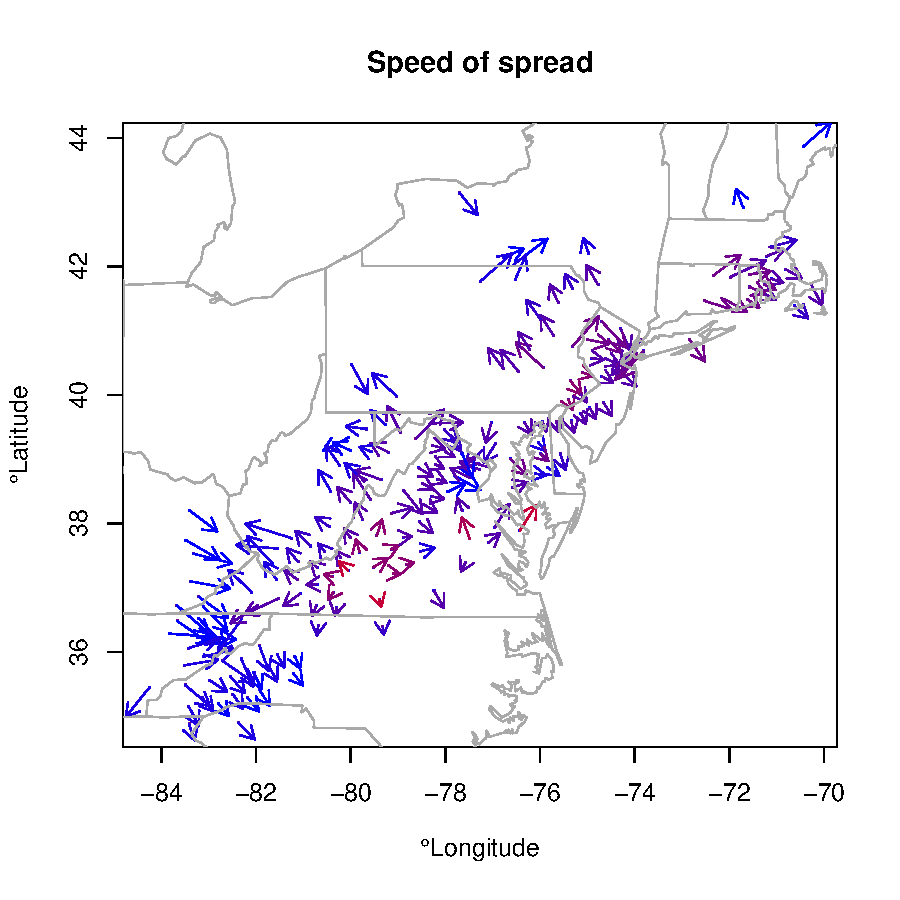
\includegraphics{invasionSpeed_doc-009}
\end{center}
\caption{gradient plot for \code{localgrad} object}
\label{grad}
\end{figure}

\section{Detecting long-range jumps}

The \pkg{invasionSpeed} package identifies candidate locations for long-range jumps in two ways. The first is the Rayleigh test (Jammalamadaka and Sengupta, 2001), and the second is a direct test using Gaussian process gradient models (Goldstein et al., 2018; Banerjee and Gelfand, 2006).

\subsection{Rayleigh test}

The Rayleigh test is a statistical test of whether a circular distribution is random or non-random. When applied to the gradients of spread near a point, a non-random distribution implies a potential long range spread through that point. \code{longrange.localgrad} function conducts Rayleigh test to the gradients from the class \code{"localgrad"} and points out candidate locations on the map.


\begin{Schunk}
\begin{Sinput}
> plotgrad(out.grad,cex=1,pch=".",database="state")
> out.longrange = longrange.localgrad(out.grad,add=TRUE)
\end{Sinput}
\end{Schunk}
In Figure \ref{rayleigh}, the black square dots represent candidate locations for long-range jumps. \code{longrange.localgrad} function tests long range jumps for a given radius (61.84688{\tt km} in this example). User can specify the radius of jumps to perform the Rayleigh test using \code{r} option in the \code{longrange.localgrad} function. Otherwise, a default value is used for testing.


\begin{figure}
\begin{center}
\begin{Schunk}
\begin{Soutput}
Long range jumps tested for  61.84688 km.
\end{Soutput}
\end{Schunk}
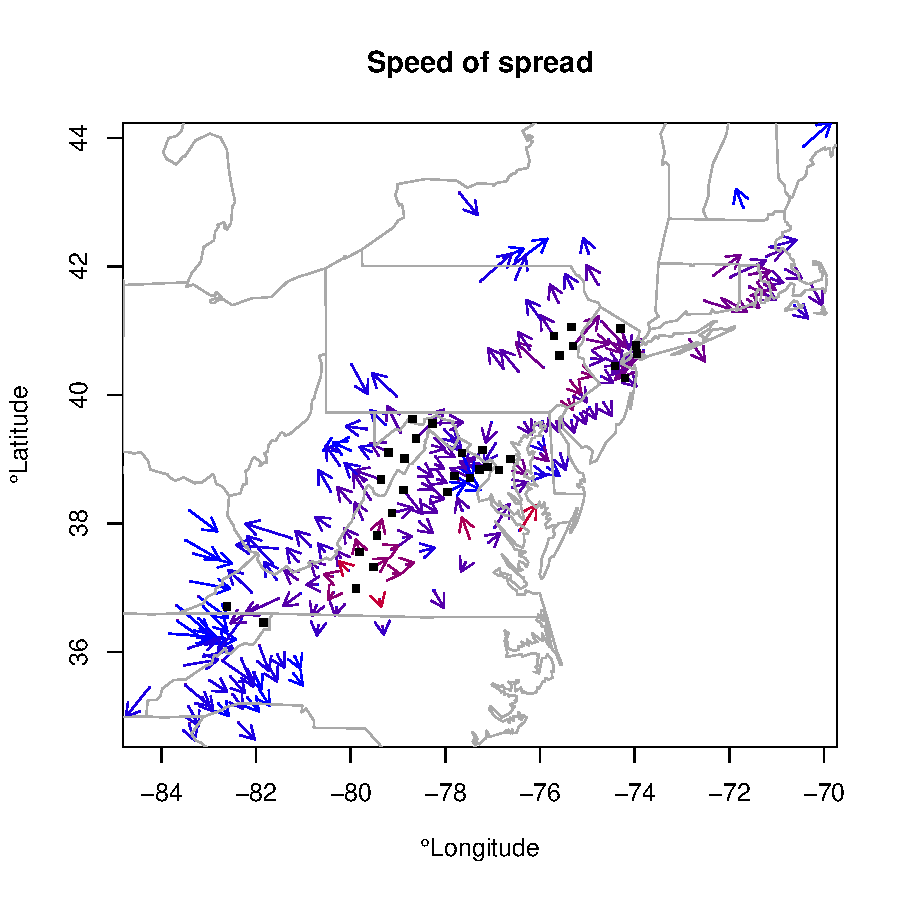
\includegraphics{invasionSpeed_doc-011}
\end{center}
\caption{Detecting long-range jump using the Rayleigh test}
\label{rayleigh}
\end{figure}

\subsection{Radial expansion of gradient models}

\code{jump.scan} function directly tests if there is significant radial expansion around a point. For each spatial location, the \code{jump.scan} function tests the gradient normal on four sides of a square with sides of length \code{r}. As a  heuristic we can flag the location as a potential site of a long-range jump if the spread is significantly out of at least two sides of the box. We can plug in parameter estimates for the Gaussian process gradient model using the posterior samples from class \code{"localgrad"}.

\begin{Schunk}
\begin{Sinput}
> par.mean = apply(out.grad$post.samp,2,mean)
> out.jump <- jump.scan(dates=dates, coord.longlat=coord,
+                       params = par.mean, Albers= c(29.5,45.5) )
> class(out.jump)
\end{Sinput}
\begin{Soutput}
[1] "jump.scan"
\end{Soutput}
\end{Schunk}

The \code{jump.scan} function returns an object of class \code{"jump.scan"}. The \code{plotboxes} function draws boxes, which represent the detected long-range jumps from class \code{"jump.scan"}. The \code{num.sides} option decides the number of significant sides to be drawn.

\begin{Schunk}
\begin{Sinput}
> plotgrad(out.grad,cex=1,pch=".",database="state")
> plotboxes(object = out.jump, num.sides = 2,method="box")
\end{Sinput}
\end{Schunk}

We can check candidate locations for long-range jumps (center of the boxes) from Figure \ref{GPjump1}. In addition, \code{plotboxes} function prints the tested radius of the jumps (61.84688{\tt km} in this example). User can specify the radius of jumps using the \code{r} option in the \code{jump.scan} function; otherwise a default value is used for testing.

\begin{figure}
\begin{center}
\begin{Schunk}
\begin{Soutput}
Long range jumps tested for  61.84688 km.
\end{Soutput}
\end{Schunk}
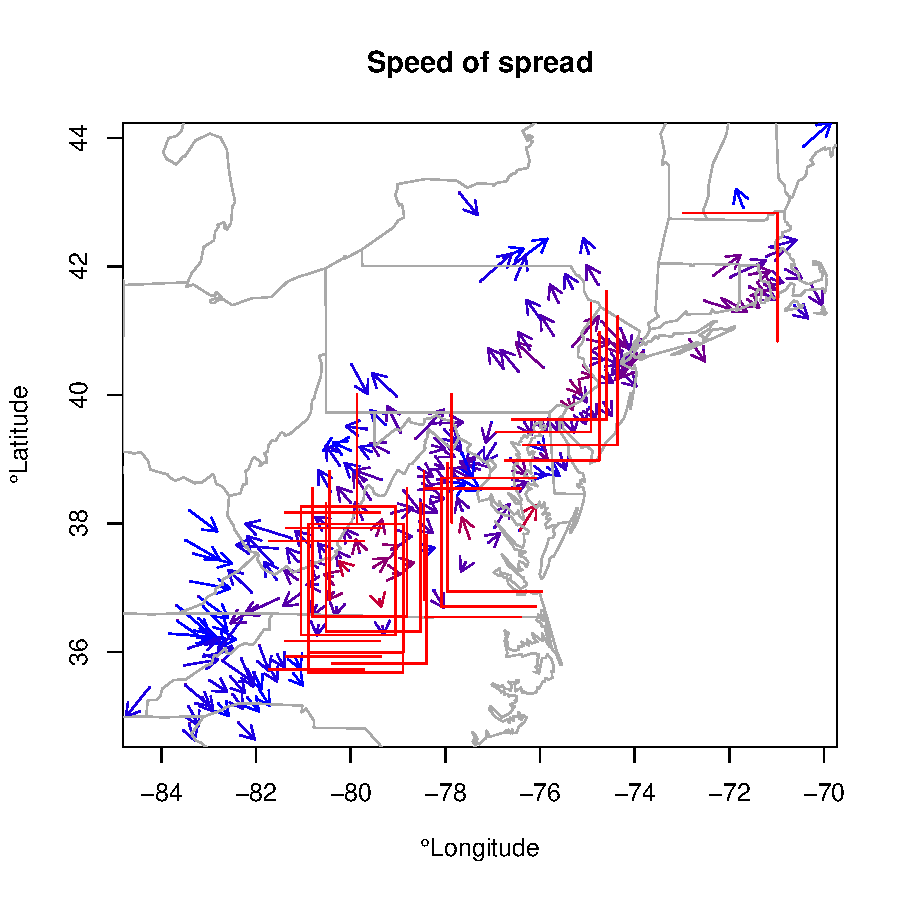
\includegraphics{invasionSpeed_doc-014}
\end{center}
\caption{Detecting long-range jump using a Gaussian process gradient model}
\label{GPjump1}
\end{figure}

\begin{Schunk}
\begin{Sinput}
> plotgrad(out.grad,cex=1,pch=".",database="state")
> plotboxes(object = out.jump, num.sides = 2,method="arrow",point=TRUE)
\end{Sinput}
\end{Schunk}
We can draw arrow plots by specifying \code{method} as \code{arrow}. In Figure \ref{GPjump2}, we plot candidate locations and arrows according to the detected direction of long-range jumps.

\begin{figure}
\begin{center}
\begin{Schunk}
\begin{Soutput}
Long range jumps tested for  61.84688 km.
\end{Soutput}
\end{Schunk}
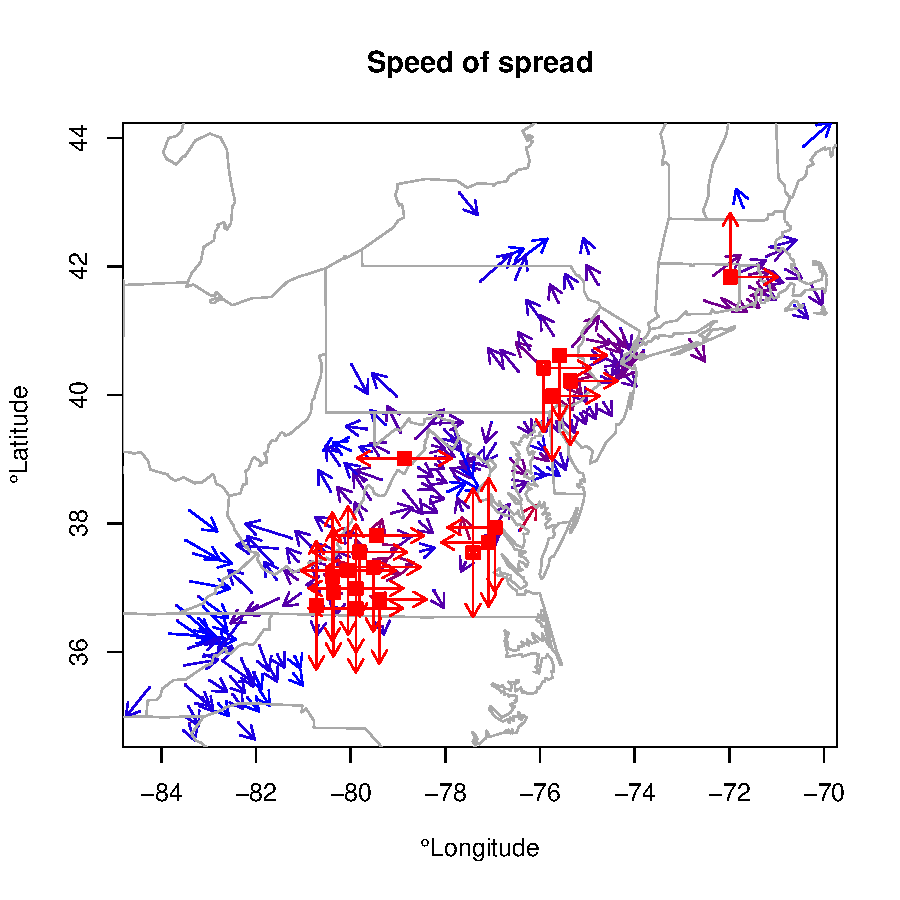
\includegraphics{invasionSpeed_doc-016}
\end{center}
\caption{Detecting long-range jump using a Gaussian process gradient model}
\label{GPjump2}
\end{figure}



\section*{References}
\begin{description}

\item Banerjee, S., Gelfand, A., and Sirmans, C., 2003, Directional rates of change under spatial process models, Journal of the American Statistical Association, 98(464):946-954.

\item Banerjee, S. and Gelfand, A., 2006, Bayesian wombling: Curvilinear gradient assessment under spatial process models, Journal of the American Statistical Association, 101(476):1487-1501.

\item Goldstein, J., Jaewoo Park, Haran, M., Liebhold, A., and Bjornstad, O. N., 2018, Quantifying Spatio-Temporal Variation of Invasion Spread, arXiv preprint arXiv:1506.02685v3.

\item Jammalamadaka, S. R. and Sengupta, A., 2001, Topics in circular statistics. World Scientific.

\end{description}
\end{document}
